\section{Simulations}
In this part, simulations of the selected topology will be provided. Simulations will be provided in three parts, in the first part we provide three-phase diode rectifier simulations and results. In the second part buck converter results and simulations are provided. In the last part, the circuit as a whole will be examined.

\subsection{Simulations of Three Phase Diode Rectifier}

In the Figure \ref{Schematic3diode} below, schematic of Simulink simulation can be observed. This simulation is constructed with a single resistance at the output. This simulation does not contain line impedances, and diodes are ideal.

\begin{center}
\begin{figure}[H]
\centering
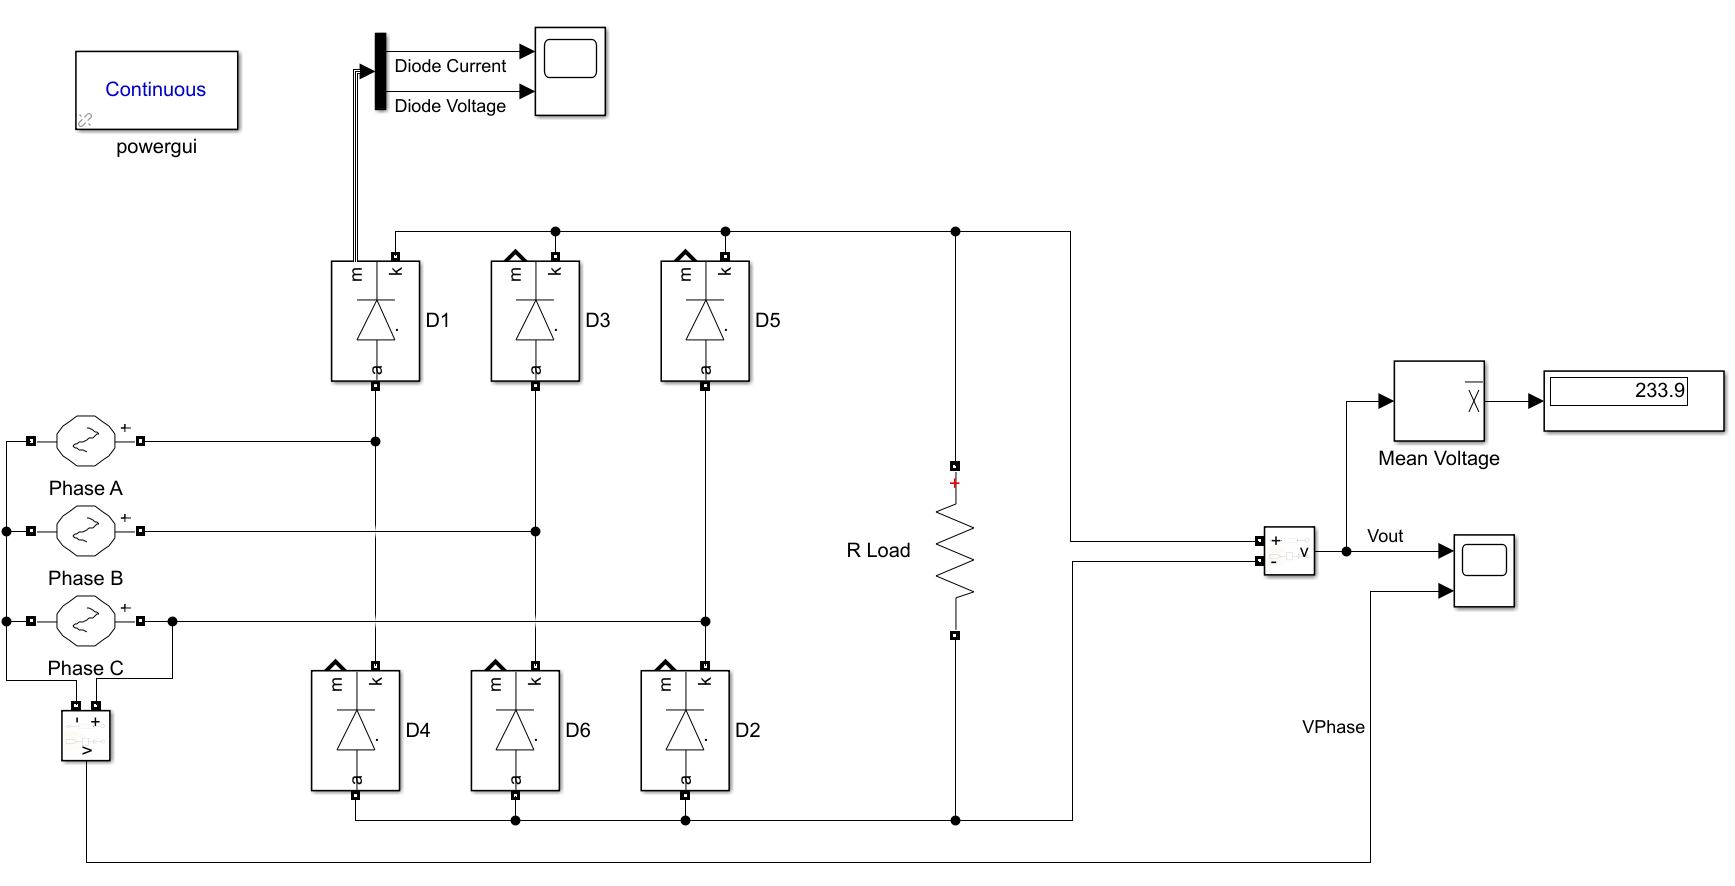
\includegraphics [width= 15 cm ]{diodetopology}
\caption{Schematic of Three Phase Diode Rectifier}
\label{Schematic3diode}
\end{figure}
\end{center}

It is given that the output voltage of the whole converter $V_{max}$ must be less than $180V_{dc}$. We limited the duty cycle of buck converter to 80\%. Then, $V_{rectifier,av}$ can be calculated as below formula.

\[V_{in,buck} = V_{rec,ac} = \frac{V_{out}}{D}=225V\]

$V_{RMS}$ can be calculated as:

\[V_s = 225\frac{\pi}{3\sqrt{6}}=96.2 V_{rms}\]

So, the input voltage was chosen as $100V_{rms}$

In the Figure \ref{Voltage3diode} below, input phase voltage and output voltage can be observed.
\begin{center}
\begin{figure}[H]
\centering
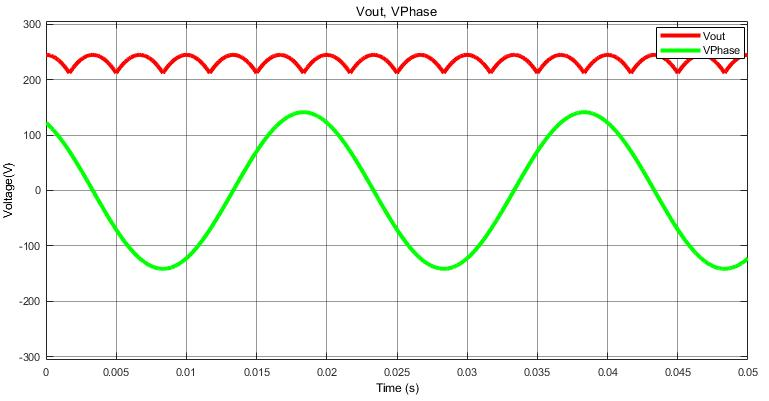
\includegraphics [width= 12 cm ]{voltageout}
\caption{Voltage Output and Voltage Input of Three Phase Diode Rectifier}
\label{Voltage3diode}
\end{figure}
\end{center}

Input voltage of a three-phase diode rectifier has frequency of 50, Turkish Grid Frequency. However, as we observe in the output, output has six times of input frequency. Thus, this topology can be named as six pulse diode rectifier. Output voltage ripple is respectively low in this case. It can be simulated as 32.8 V. Moreover, this topology does not have triplen harmonics in input current. This results in lower THD, and better power quality. THD of this topology is simulated as 31.8\%

Input and output current waveforms can be observed from Figure \ref{Current3diode} below.

\begin{center}
\begin{figure}[H]
\centering
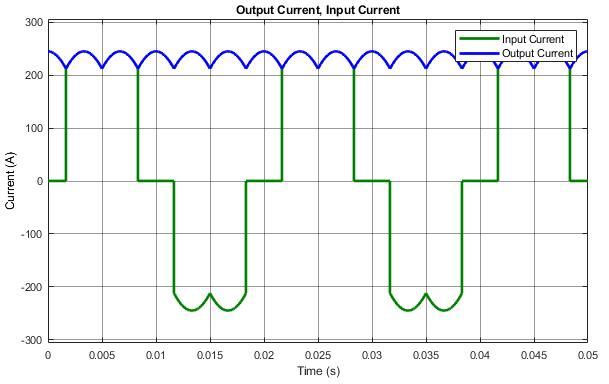
\includegraphics [width= 12 cm ]{inputcurrent}
\caption{Input Current and Output Current of Three Phase Diode Rectifier}
\label{Current3diode}
\end{figure}
\end{center}

Component selection will be based on stresses and limits. In the Figure \ref{Diode3diode} below, diode stresses can be observed.

\begin{center}
\begin{figure}[H]
\centering
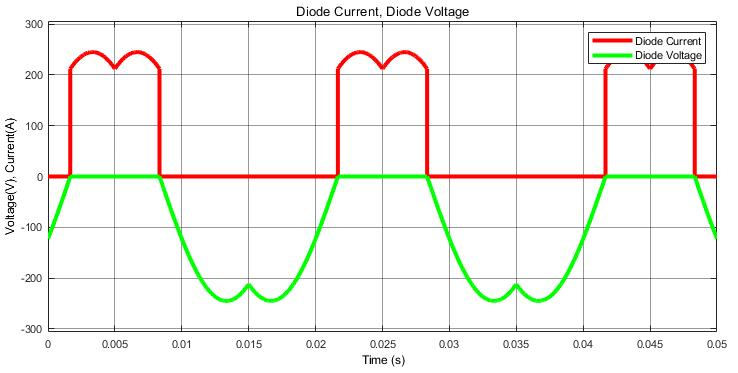
\includegraphics [width= 12 cm ]{currentdiode}
\caption{Diode Current and Diode Voltage of a Diode}
\label{Diode3diode}
\end{figure}
\end{center}

It is obvious that our diodes have to be able to carry peak current of 250A. However, this stress is for the ideal case with output resistance of 1\ohm. This value will be less when we add the buck converter, and the DC Machine. Also, our diodes should have reverse voltage of minimum -250V.

\subsection{Simulations of Buck Converter}
The Simulink simulation schematic of the Buck Converter circuit topology is given in Figure \ref{voltcurrentbuckout}. The topology is simulated to observe the output voltage and current waveforms, diode current and voltage waveforms and MOSFET voltage and current waveforms.

In the simulations, the switching frequency of the MOSFET is chosen 1 kHz with 10\% duty cycle. Since initially dc motor is at standstill, there is no back emf produced by the motor, which will limit the output current of the Buck Converter. Therefore, we should be careful about the start-up current of the dc motor. In order to limit the output current at start-up, we have decided to initially set the duty cycle of the control signal to be 0.1 . Thus, it is ensured that the output current does not exceed the rated current of the dc motor, which is provided 23.4 A. We plan to steadily increase the duty cycle of the control signal from 0.1 (10\%) to 0.8 (80\%) in a finite duration until the back emf of the motor builts up while it is reaching its rated speed, and hence reach steady state condition. Thereafter, we can control the output dc voltage of the converter circuit to obtain variable DC output converter. The input voltage is applied from a dc voltage source with 225 V as computed in the subsection 4.1. Since the dc motor itself is a big RL load, it is thought to be unnecessary to add an LC filter at the output for the Buck Converter. Hence, we have modelled the buck converter without LC filter at the output. The output of the Buck Converter circuit is loaded with the resistance (R) and inductance (L) ratings of the DC Motor to be driven. A dc voltage source representing the back emf voltage of the dc motor is also added at the output. However, it is set to 0.1 V in order to obtain the start-up current and voltage waveforms of the output load, MOSFET and freewheeling diode. The observed peak and average values of the current and voltage waveforms across the MOSFET and diode in simulations will be used in the component selection part to select the components with the suitable ratings to our circuit.

\begin{center}
\begin{figure}[H]
\centering
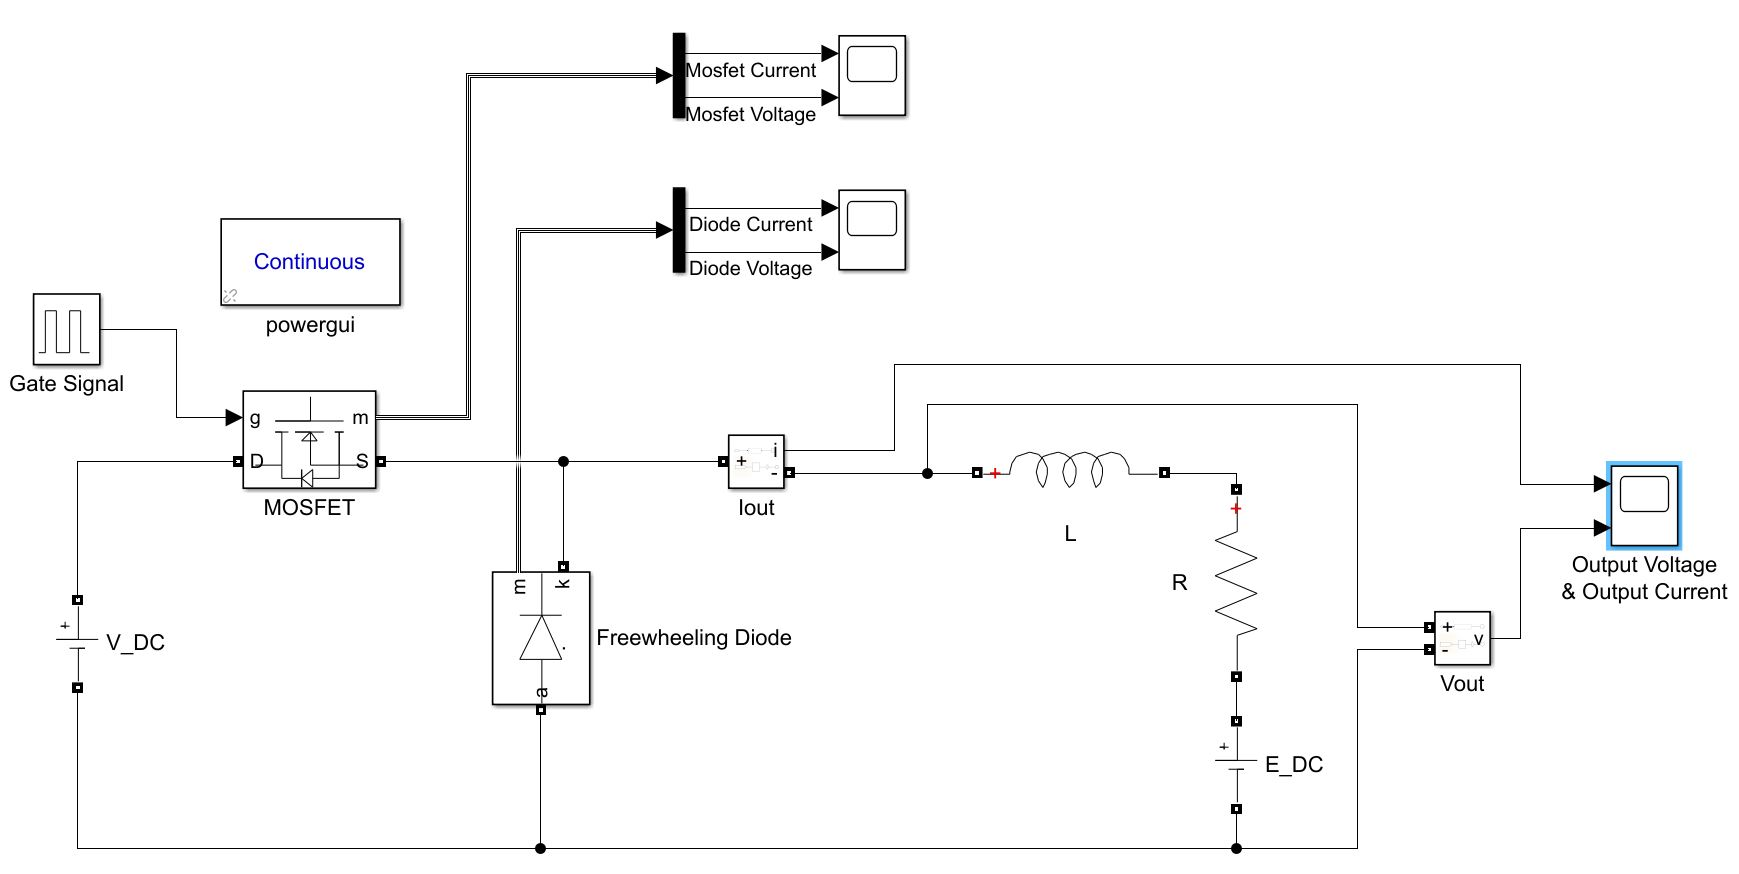
\includegraphics [width= 12 cm ]{voltcurrentbuckout}
\caption{Schematic of Buck Converter}
\label{voltcurrentbuckout}
\end{figure}
\end{center}

In the Figure \ref{buckvoltagecurrentout}, the output voltage and current waveforms of the Buck Converter circuit, obtained from simulations, are given.

At the output of the Buck Converter, a square wave voltage waveform is observed. The ripple in the output voltage is measured to be close to 225 V. However, the ripple in the output current of the circuit is quite small.
\begin{center}
\begin{figure}[H]
\centering
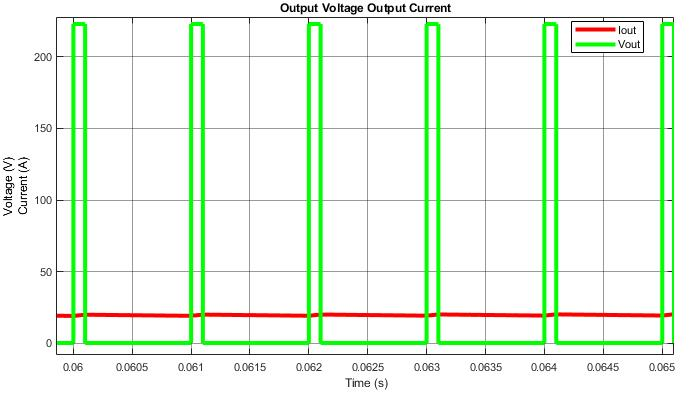
\includegraphics [width= 12 cm ]{buckvoltagecurrentout}
\caption{Buck Converter Output Voltage and Output Current Waveforms}
\label{buckvoltagecurrentout}
\end{figure}
\end{center}

MOSFET voltage and current waveforms are given in Figure \ref{mosfetcurrvolt} below.

\begin{center}
\begin{figure}[H]
\centering
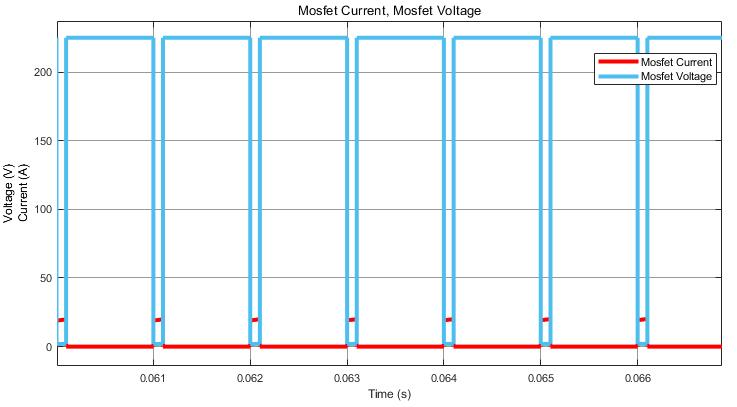
\includegraphics [width= 12 cm ]{mosfetcurrvolt}
\caption{MOSFET Voltage and Current Waveforms}
\label{mosfetcurrvolt}
\end{figure}
\end{center}

The Figure \ref{freediodecurrvolt} shows the voltage and current waveforms across the freewheeling diode.
\begin{center}
\begin{figure}[H]
\centering
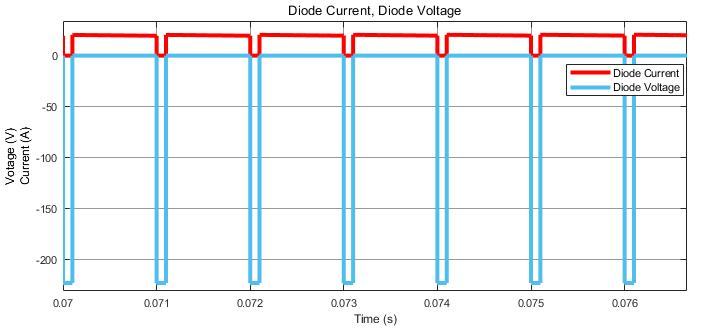
\includegraphics [width= 12 cm ]{freediodecurrvolt}
\caption{Freewheeling Diode Voltage and Current Waveforms}
\label{freediodecurrvolt}
\end{figure}
\end{center}

\subsection{Simulations of Rectifier \& Buck Converter}

In the Figure \ref{diodebuck} below, we can observe the whole circuit consists of diode rectifier and buck converter. In the schematic, we used an RL load with dc voltage, it is basically a motor model. Displays show average values of diode voltage and inputs. This values are critical for component selection.

\begin{center}
\begin{figure}[H]
\centering
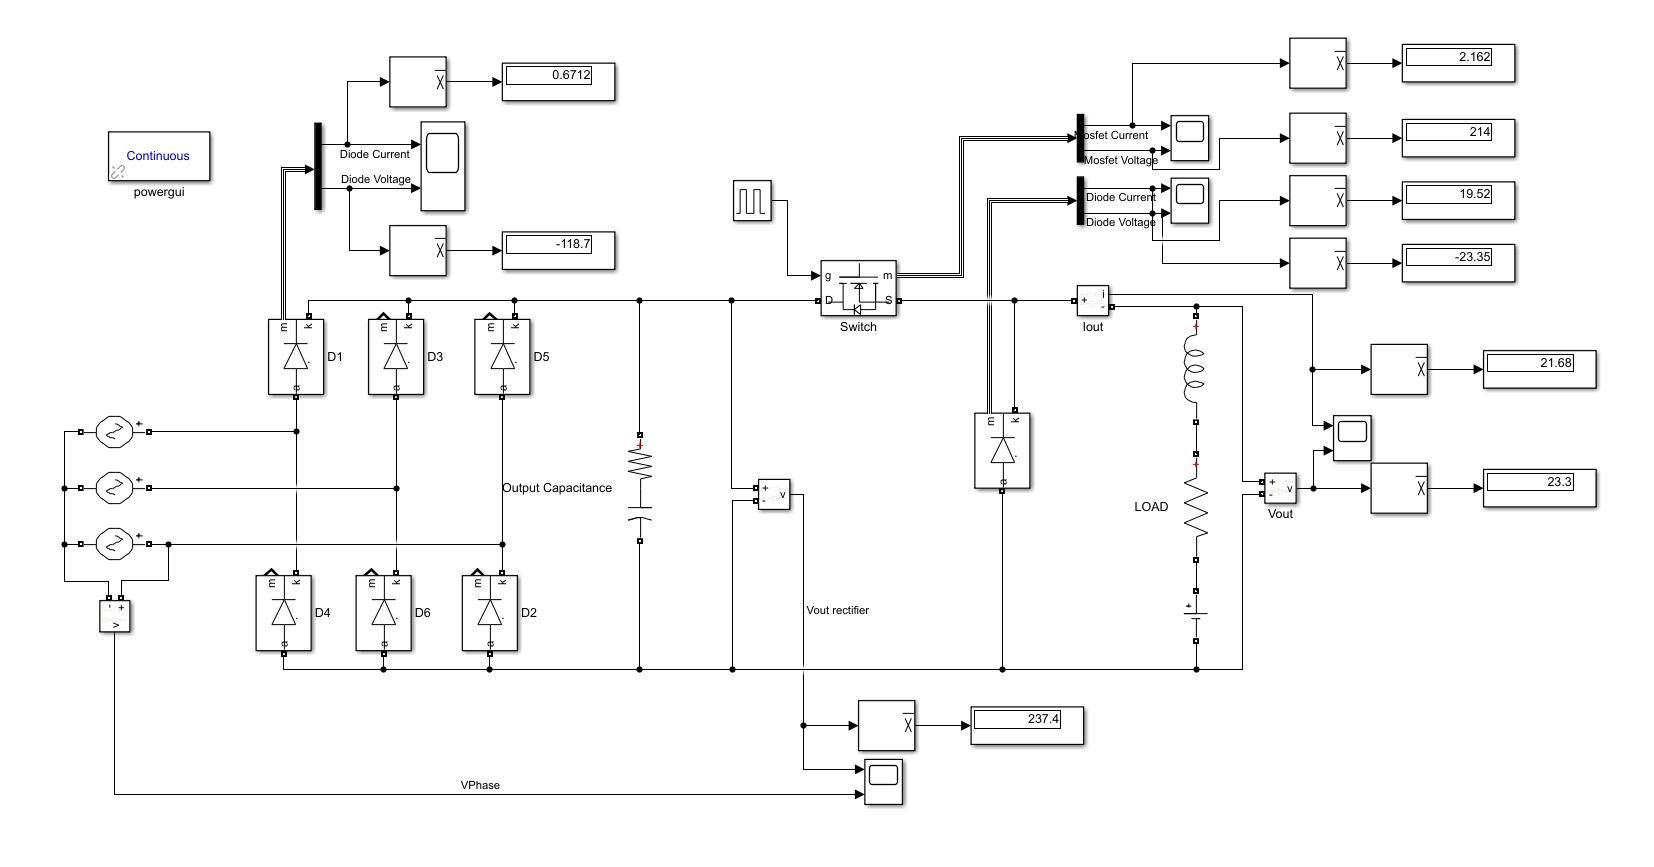
\includegraphics [width= 12 cm ]{diodebuck}
\caption{Schematic of Whole Circuit}
\label{diodebuck}
\end{figure}
\end{center}

In the Figure below \ref{wholeoutput}, output voltage and current for start up can be observed. It is taken at duty cycle of 0.1

\begin{center}
\begin{figure}[H]
\centering
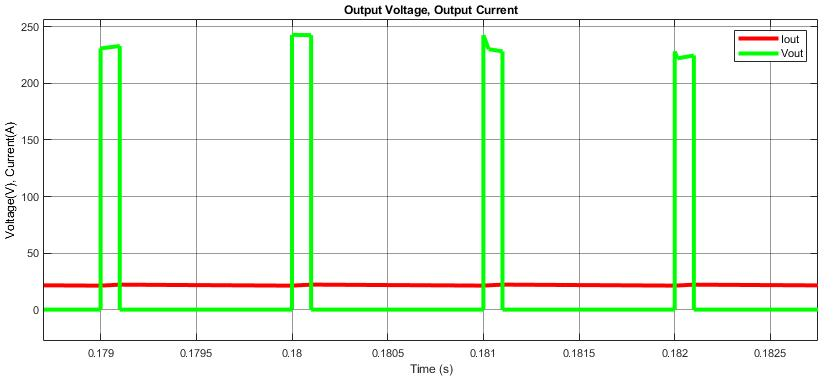
\includegraphics [width= 12 cm ]{wholeoutput}
\caption{Output Voltage and Current Waveforms of Converter}
\label{wholeoutput}
\end{figure}
\end{center}

In the Figure \ref{inputdiodewave} below, we can see transient waveform of the input diode. At start-up, maximum current is around 24 Amperes, and reverse voltage is around -250 Volts.

\begin{center}
\begin{figure}[H]
\centering
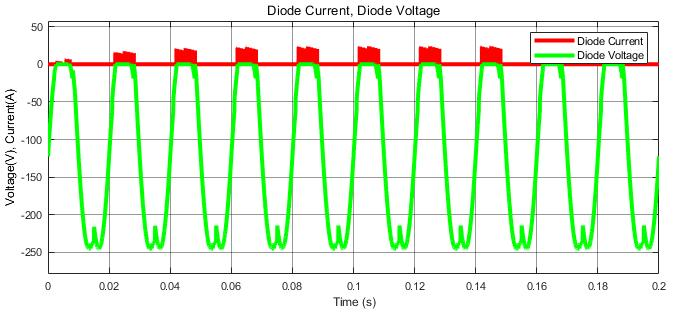
\includegraphics [width= 12 cm ]{inputdiodewave}
\caption{Rectifier Diode Voltage and Current Waveforms}
\label{inputdiodewave}
\end{figure}
\end{center}

In the Figure \ref{wholemosfet} below, we can observe MOSFET stresses, average current is around 3 Amperes and blocking voltage is around 214 Volts at start-up.
\begin{center}
\begin{figure}[H]
\centering
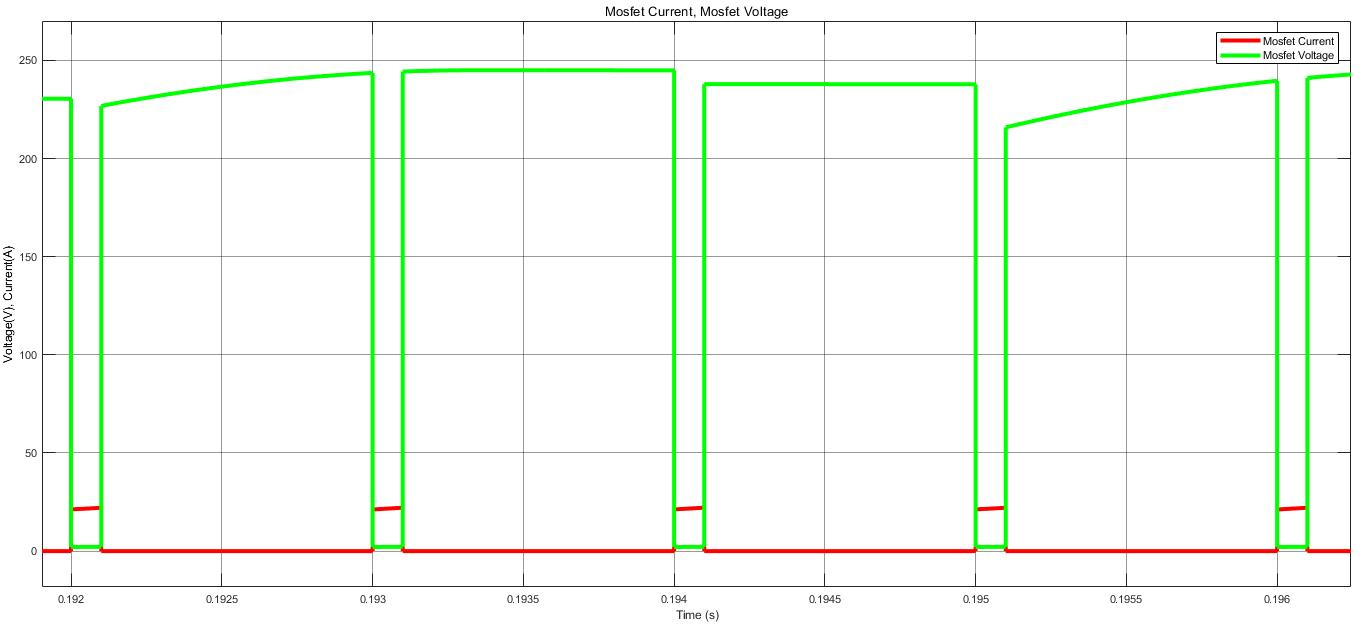
\includegraphics [width= 12 cm ]{wholemosfet}
\caption{MOSFET Voltage and Current Waveforms at Start-Up, D=10\%}
\label{wholemosfet}
\end{figure}
\end{center}

In the Figure \ref{diodesteady} below, we can observe the freewheeling diode stresses, average current is around 25 Amperes and blocking voltage is around 220 Volts at start-up.
\begin{center}
\begin{figure}[H]
\centering
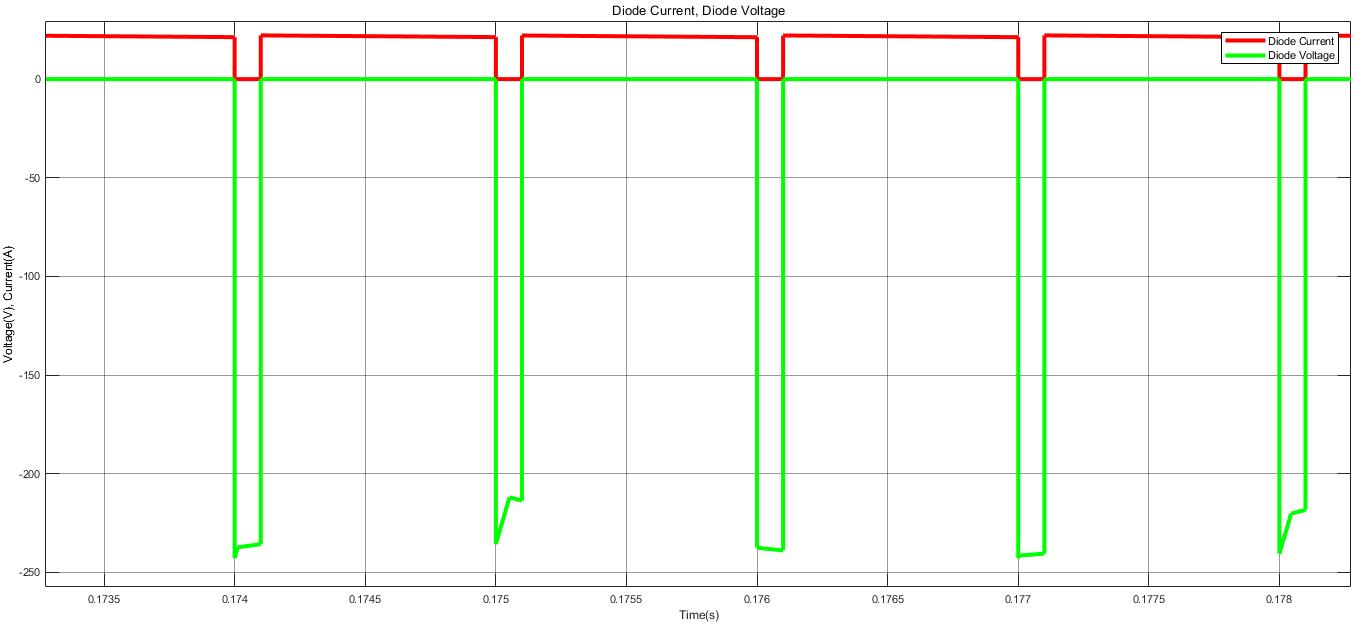
\includegraphics [width= 12 cm ]{diodesteady}
\caption{Freewheeling Diode Voltage and Current Waveforms at Start-Up, D=10\%}
\label{diodesteady}
\end{figure}
\end{center}

In the Figure \ref{diodefinal} below, we can observe the freewheeling diode stresses, average current is around 20 Amperes and the reverse voltage is around 25 Volts at steady-state.
\begin{center}
\begin{figure}[H]
\centering
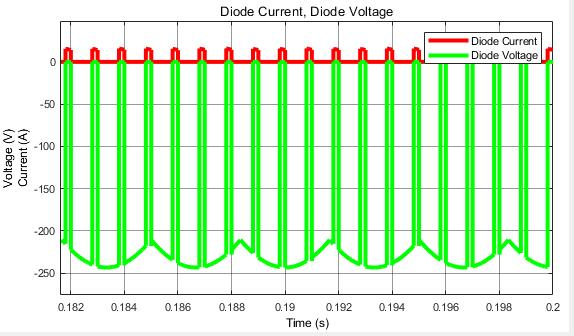
\includegraphics [width= 12 cm ]{finalfwd}
\caption{Freewheeling Diode Voltage and Current Waveforms at Steady State, D=80\%}
\label{diodefinal}
\end{figure}
\end{center}

In the Figure \ref{mosfetfinal} below, we can observe the MOSFET stresses, average current is around 12 Amperes and the reverse voltage is around 50 Volts at steady-state.
\begin{center}
\begin{figure}[H]
\centering
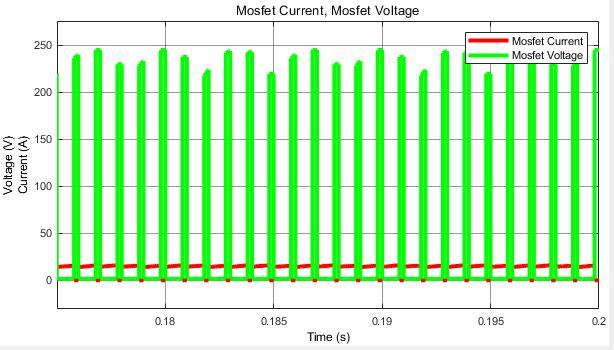
\includegraphics [width= 12 cm ]{finalmosfet}
\caption{MOSFET Voltage and Current Waveforms at Steady State, D=80\%}
\label{mosfetfinal}
\end{figure}
\end{center}

Simulations show that, critical points that need attention is:
\begin{itemize}
    \item At start-up, current of freewheeling diode and voltage of MOSFET is critical. We paid attention when we select the components.
    \item At steady-state, voltage of freewheeling diode and rectifier's diode current is critical. Also, MOSFET's current is critical. We paid attention to these parameters 
\end{itemize}





